%%%%%%%%%%%%%%%%%%%%%%%%%%%%%%%%%%%%%%%%%%%%%%%%%%%%%%%%%%%%%%%
%
% Welcome to Overleaf --- just edit your LaTeX on the left,
% and we'll compile it for you on the right. If you open the
% 'Share' menu, you can invite other users to edit at the same
% time. See www.overleaf.com/learn for more info. Enjoy!
%
%%%%%%%%%%%%%%%%%%%%%%%%%%%%%%%%%%%%%%%%%%%%%%%%%%%%%%%%%%%%%%%

% Inbuilt themes in beamer
\documentclass{beamer}

% Theme choice:
\usetheme{CambridgeUS}
\usepackage{amsmath}
\usepackage{mathtools}
\newcommand\laplace{\ensuremath{\stackrel{\mathclap{\mbox{$\mathcal{L}$}}}{\longleftrightarrow}}}
\newcommand\laplaceinv{\ensuremath{\stackrel{\mathclap{\mbox{$\mathcal{L}^{-1}$}}}{\longleftrightarrow}}}
\providecommand{\pr}[1]{\ensuremath{\Pr\left(#1\right)}}
\providecommand{\cdf}[2]{\ensuremath{\text{F}_{#1}\left(#2\right)}}
\providecommand{\erf}[1]{\ensuremath{\text{erf}(#1)}}
\setbeamertemplate{caption}[numbered]
% Title page details: 
\title{Assignment 14} 
\author{Gautam Singh (CS21BTECH11018)}
\date{\today}

\begin{document}

% Title page frame
\begin{frame}
    \titlepage 
\end{frame}

% Outline frame
\begin{frame}{Outline}
    \tableofcontents
\end{frame}

\section{Problem}
\begin{frame}{Problem Statement}
	\textbf{(Papoulis/Pillai, Exercise 8-25)} We are given a random variable $X$ with mean $\eta$ and standard deviation $\sigma = 2$, and we wish to test the hypothesis $\eta = 8$ against $\eta = 8.7$ with $\alpha = 0.01$ using as the test statistic the sample mean $\bar{x}$ of $n$ samples.
	\begin{enumerate}
		\item Find the critical region $R_c$ of the test and the resulting $\beta$ if $n = 64$. 
		\item Find $n$ and $R_c$ if $\beta = 0.05$.
	\end{enumerate}
\end{frame}

\section{Hypothesis Testing}
\begin{frame}{Definitions}
	\begin{alertblock}{Random Variable Used}
		When using the test statistic as the mean ($\bar{X}$), we consider the random variable
		\begin{align}
			Q = \frac{\bar{X} - \eta}{\frac{\sigma}{\sqrt{n}}}
			\label{eq:Q}
		\end{align}
		We assume $\bar{X} \sim N(\eta_0 ; \frac{\sigma}{\sqrt{n}})$. Hence, $Q \sim N(\eta_q ; 0)$, where
		\begin{align}
			\eta_q = \frac{\eta - \eta_0}{\frac{\sigma}{\sqrt{n}}}
			\label{eq:eta-q}
		\end{align}
		Observe that for the null hypothesis $H_0: \eta = \eta_0$, we have $Q \sim N(0; 1)$ so we can use the standard normal percentiles.
	\end{alertblock}
\end{frame}

\section{Solution}
\begin{frame}{Solution}
	Note that in this solution, writing $\pr{\ldots | H_0}$ denotes that the hypothesis $H_0$ is true. Also note that percentile notation is used. In particular, $z_p$ denotes the point of the $p^{th}$ percentile of the standard normal disribution.
	\begin{enumerate}
		\item[1] For $\eta > \eta_0$, the critical region is the half-line $q > c$, where 
			\begin{align}
				\pr{Q > c | H_0} &= \alpha \\
				\implies c &= q_{1 - \alpha} \\
				\implies c &= \eta + z_{1 - \alpha}\frac{\sigma}{\sqrt{n}} = 8 + 2.326 \times \frac{2}{8} = 8.58
				\label{eq:r-c}
			\end{align}
			Hence, $R_c$ is given by $\bar{x} > 8.58$ (refer Figure \eqref{fig:graph}). Now, if $H_1: \eta > \eta_0$, then
			\begin{align}
				\eta_q = \frac{8.7 - 8}{\frac{2}{8}} = 2.8
				\label{eq:new-eta}
			\end{align}
	\end{enumerate}
\end{frame}

\begin{frame}
	\begin{figure}
		\centering
		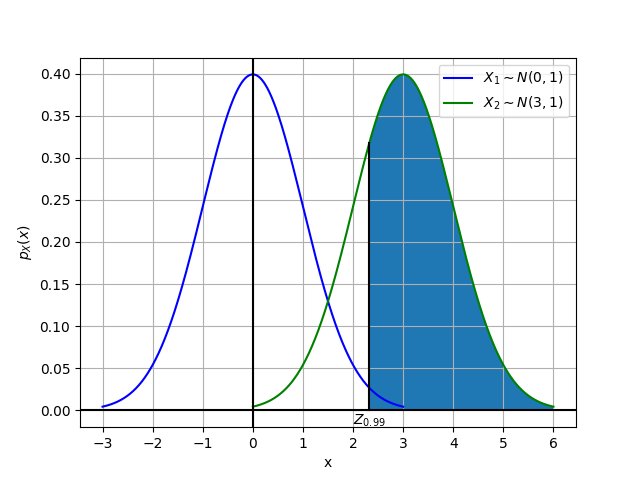
\includegraphics[height=0.8\textheight]{figs/14_1.png}
		\caption{Critical region where null hypothesis is rejected.}
		\label{fig:graph}
	\end{figure}
\end{frame}

\begin{frame}
	\begin{enumerate}
		\item[1] (Cont'd...) $\beta$ is a function of $\eta$ given by
			\begin{align}
				\beta(\eta) &= \pr{Q \notin R_c | H_1} = \pr{Q < c} \\
				&= \erf{z_{1 - \alpha} - \eta_q} = 0.32
				\label{eq:beta-eta}
			\end{align}
		\item[2] Proceeding in reverse from \eqref{eq:beta-eta}, we have from the definition of $\beta$, 
			\begin{align}
				z_{1 - \alpha} - \eta_q &= z_{\beta} \\
				\implies \eta_q &= z_{1 - \alpha} - z_{\beta} \\
				&= z_{0.99} - z_{0.05} = 4.97
				\label{eq:eta-q-rev}
			\end{align}
			However, assuming that $\beta(8.7) = 0.05$, we can also use \eqref{eq:eta-q} to get 
			\begin{align}
				n = \left(\frac{\sigma\eta_q}{\eta - \eta_0}\right)^2 = 129
				\label{eq:n}
			\end{align}
			Thus, using \eqref{eq:r-c}, we get 
			\begin{align}
				c = 8 + z_{0.99}\frac{2}{\sqrt{129}} = 8.41
				\label{eq:c-ans}
			\end{align}
	\end{enumerate}
\end{frame}

\end{document}
